%	This LaTeX file is written by Zhiyang Ong as a template for writing reports.

%	The MIT License (MIT)

%	Copyright (c) <2014> <Zhiyang Ong>

%	Permission is hereby granted, free of charge, to any person obtaining a copy of this software and associated documentation files (the "Software"), to deal in the Software without restriction, including without limitation the rights to use, copy, modify, merge, publish, distribute, sublicense, and/or sell copies of the Software, and to permit persons to whom the Software is furnished to do so, subject to the following conditions:

%	The above copyright notice and this permission notice shall be included in all copies or substantial portions of the Software.

%	THE SOFTWARE IS PROVIDED "AS IS", WITHOUT WARRANTY OF ANY KIND, EXPRESS OR IMPLIED, INCLUDING BUT NOT LIMITED TO THE WARRANTIES OF MERCHANTABILITY, FITNESS FOR A PARTICULAR PURPOSE AND NONINFRINGEMENT. IN NO EVENT SHALL THE AUTHORS OR COPYRIGHT HOLDERS BE LIABLE FOR ANY CLAIM, DAMAGES OR OTHER LIABILITY, WHETHER IN AN ACTION OF CONTRACT, TORT OR OTHERWISE, ARISING FROM, OUT OF OR IN CONNECTION WITH THE SOFTWARE OR THE USE OR OTHER DEALINGS IN THE SOFTWARE.

%	Email address: echo "cukj -wb- 23wU4X5M589 TROJANS cqkH wiuz2y 0f Mw Stanford" | awk '{ sub("23wU4X5M589","F.d_c_b. ") sub("Stanford","d0mA1n"); print $5, $2, $8; for (i=1; i<=1; i++) print "6\b"; print $9, $7, $6 }' | sed y/kqcbuHwM62z/gnotrzadqmC/ | tr 'q' ' ' | tr -d [:cntrl:] | tr -d 'ir' | tr y "\n"

%%%%%%%%%%%%%%%%%%%%%%%%%%%%%%%%%%%%%%%%%%%%%%









%%%%%%%%%%%%%%%%%%%%%%%%%%%%%%%%%%%%%%%%%%%%%%
%	Preamble.
\documentclass[letterpaper,12pt]{report}
%%%%%%%%%%%%%%%%%%%%%%%%%%%%%%%%%%%%%%%%%%%%%
%
%	Importing LaTeX source files, without quoting the ".tex" extension.
%
%%%%%%%%%%%%%%%%%%%%%%%%%%%%%%%%%%%%%%%%%%%%%

%%%%%%%%%%%%%%%%%%%%%%%%%%%%%%%%%%%%%%%%%%%%%
%	File containing the LaTeX preamble.
% This is written by Zhiyang Ong as the preamble for all his LaTeX documents.
%
% It includes a list of LaTeX packages that he commonly uses to typeset LaTeX documents.

%	The MIT License (MIT)

%	Copyright (c) <2014> <Zhiyang Ong>

%	Permission is hereby granted, free of charge, to any person obtaining a copy of this software and associated documentation files (the "Software"), to deal in the Software without restriction, including without limitation the rights to use, copy, modify, merge, publish, distribute, sublicense, and/or sell copies of the Software, and to permit persons to whom the Software is furnished to do so, subject to the following conditions:

%	The above copyright notice and this permission notice shall be included in all copies or substantial portions of the Software.

%	THE SOFTWARE IS PROVIDED "AS IS", WITHOUT WARRANTY OF ANY KIND, EXPRESS OR IMPLIED, INCLUDING BUT NOT LIMITED TO THE WARRANTIES OF MERCHANTABILITY, FITNESS FOR A PARTICULAR PURPOSE AND NONINFRINGEMENT. IN NO EVENT SHALL THE AUTHORS OR COPYRIGHT HOLDERS BE LIABLE FOR ANY CLAIM, DAMAGES OR OTHER LIABILITY, WHETHER IN AN ACTION OF CONTRACT, TORT OR OTHERWISE, ARISING FROM, OUT OF OR IN CONNECTION WITH THE SOFTWARE OR THE USE OR OTHER DEALINGS IN THE SOFTWARE.

%	Email address: echo "cukj -wb- 23wU4X5M589 TROJANS cqkH wiuz2y 0f Mw Stanford" | awk '{ sub("23wU4X5M589","F.d_c_b. ") sub("Stanford","d0mA1n"); print $5, $2, $8; for (i=1; i<=1; i++) print "6\b"; print $9, $7, $6 }' | sed y/kqcbuHwM62z/gnotrzadqmC/ | tr 'q' ' ' | tr -d [:cntrl:] | tr -d 'ir' | tr y "\n"

%%%%%%%%%%%%%%%%%%%%%%%%%%%%%%%%%%%%%%%%%%%%%%%%%%

% Importing some standard LaTeX packages.

% To enable standard LaTeX processing for graphics. It enables PDF, JPEG, PNG, and TIFF graphics files to be included in the LaTeX document.
\usepackage{graphicx}
% For better typesetting of mathematical expressions, from the American Mathematical Society (AMS).
\usepackage{amsmath}
% For better typesetting of mathematical expressions, from the American Mathematical Society (AMS). This package includes mathematical symbols for the ``amsmath'' package.
\usepackage{amssymb}
% For better typesetting of mathematical proofs (for theorems and colloraries), from the American Mathematical Society (AMS).
\usepackage{amsthm}
%	Create definitions for new theorems, axioms, colloraries.
	\newtheorem{theorem}{Theorem}[chapter]
	\newtheorem{axiom}{Axiom}[chapter]
	\newtheorem{corollary}{Corollary}[chapter]
	\newtheorem{lemma}{Lemma}[chapter]
	\newtheorem{Rule}{Rule}[chapter]
	\newtheorem{law}{Law}[chapter]
	\newtheorem{principle}{Principle}[chapter]
% To change the style of newly defined theorems.
%		\usepackage{theorem}


% For better typesetting of tables (and arrays).
\usepackage{array}
% For creating tables without vertical separators.
%		\usepackage{booktabs}
% To control line spacing in LaTeX documents.
\usepackage{setspace}
% To modify the spacing between words and letters.
%		\usepackage{microtype}
% To change the dimensions of the page(s).
%\usepackage[margin=1.5cm,vmargin={0pt,1cm},nohead]{geometry}
\usepackage[margin=1.5cm,vmargin={1.5cm,2cm}]{geometry}
% Use the packages needed to typeset algorithms. I can also use the combined ``algorithms'' bundle.
\usepackage{algorithm}
\usepackage{algorithmic}
% The listings package is a source code printer for LaTeX. You can typeset stand alone files as well as listings with an environment similar to verbatim as well as you can print code snippets using a command similar to \verb. Many parameters control the output and if your preferred programming language isn�t already supported, you can make your own definition.
\usepackage{listings}
% Use the ``clrscode3e'' LaTeX package to typeset algorithms like CLRS
%	\usepackage{/data/others/notes/clrscode3e}
\usepackage{/data/others/grappanotes/clrscode3e}
% Use the ``algpseudocode'' LaTeX package to typeset algorithms -- Alternate solution, not preferred
%\usepackage{algpseudocode}
% Alternative packages for typesetting algorithms.
%\usepackage{algorithm2e}
%\usepackage{algorithmicx}
%\usepackage{program}
%	To check for syntax errors in my LaTeX document.
\RequirePackage[l2tabu, orthodox]{nag}

% Concatenate adjacent references together when typeset.
% That is, cite{ref1,ref2,ref3,ref4} can appear as [12-15], instead of [12] [13] [14] [15]
\usepackage{cite}
% For automatic insertion of cross-referencing words, such as fig. for figures and eq. for equations.
%		\usepackage{cleveref}

% LaTeX support for Metafont and MetaPost logos.
\usepackage{mflogo}













% How to typeset single and double quotes for feet and inches?
% For feet, use [FEET]\textasciiacute
% For inches, use [INCHES]\textacutedbl
% For feet and inches, use [FEET]\textasciiacute\ [INCHES]\textacutedbl; force a character space between the single quote for feet and the height of the object in inches
% Don't use \textceltpal as a single quote to represent height in feet, or double \textceltpal (two concatenated \textceltpal) as a double quote to represent height in inches
% For double quotes, don't use two single quotes provided by the default settings of LaTeX. The resultant double quotes will be curly.

% The tipa package is for Phonetic Symbols -- I wanna use the \textceltpal symbol to represent a single quote, instead of using the generic ``curly'' single quote from \LaTeX (Table 10, pp.10)
\usepackage{tipa}
% The textcomp package is for Diacritics -- I wanna use the \textacutedbl symbol to represent a double quote (Table 28, pp.17), instead of using the generic ``curly'' double quotes from \LaTeX; however, when this symbol is used, I must force a character space to exist after the symbol by using the backslash followed by a character space. This package also provides the symbol for Copyleft, \textcopyleft, which is not available in LaTeX by default, and provides better looking symbols for: copyright, registered, and trademark (Table 33, pp.18). Also, it provides symbols for: \textcelsius, \textmho, \textmu, \textohm (Table 201, pp.67). It also provides symbols for Genealogical Symbols (Table 253, pp78), such as \textborn, \textdivorced, \textmarried, \textdied, and \textleaf (symbol of a leaf)... Its symbol for the Euro, EU currency, is \texteuro
\usepackage{textcomp}
% Look at \url{http://www.ctan.org/tex-archive/info/symbols/comprehensive/symbols-a4.pdf} for a list of symbols that can be used in LaTeX and its packages. Table 280, pp.88, deals with Symbol Name Clashes; hence, if the same command name refers to multiple symbols, the symbol-conflict resolution abides by this.
% In particular, check out the gensymb package (Table 197, page 67) for symbols defined to work in both math and text modes, such as \celsius, \micro, \degree, and \ohm.
% Also, check out the wasysym package (Table 198, page 67) for electrical symbols, such as that of alternating current (AC); it also provides symbols for \female, and \male (Table 212, pp.70); it also has symbols for ``Xs and Check Marks,'' which are checked boxes, \CheckedBox, squares, \Square, and crossed boxes (boxes filled with a cross), \XBox (Table 232, pp.73); it also has symbols for a clock, \clock, a Simley, \smiley, diameter, \diameter, lightning, \lightning, sun, \sun, and a tick or check mark \checked (symbol to indicate that something is correct), and a bell, \bell (Table 254, pp.78); it also has symbols for left and right turns (Table 256, pp.78), \leftturn and \rightturn; this package (Table 256, pp.78) and the arev package (Table 257, pp.78) can be used to typeset music symbols, along with Table 182, pp.62; it also has symbols for Navigation (Table 261, pp.79), such as \Forward, \RewindToStart, and \ForwardToIndex; it also has symbols for laundry (Table 262, pp.80); it also has the symbol for a heart, \Heart (Table 263, pp.80).
% In addition, check out the ifsym package (Table 199, page 67) for pulse diagram symbols; it also has symbols for weather (Table 266, pp.80), alpine and mountain climbing, such as \Summit, \Mountain, \IceMountain, \VarMountain, \Flag, \FilledHut, \Hut, \Village, and \Tent (Table 267, pp.81); it also has different symbols for clocks, such as \Interval, \StopWatchEnd, \VarClock, \showclock (to indicate the time) (Table 268, pp.81); it also has symbols for fire, letter, telephone, dice, \PaperPortrait, and \PaperLandscape. Also, has symbol for the cross to indicate that something is incorrect
\usepackage{ifsym}
% Besides, check out the keystroke package (Table 208, page 69) for symbols of Computer Keys, such as Alt, Ctrl, Del, Page down, Esc, Enter, Shift, Space Bar, and Up Arrow.
% From the dingbat package (Table 225, page 72), it has symbols for Fists, such as \rightthumbsdown and \rightthumbsup.
%\usepackage{dingbat}
% From the pifont package (Table 234, page 73), it has symbols for Circled Numbers, such as any digit that is circled, where the space in the circle can be shaded black.
% From the dictsym package (Table 277, page 84), it has symbols for dictionaries, and indicates which type of dictionary will define this term - say a medical, technical, mathematical, or judical dictionary
% The simpsons package can be used to indicate characters from {\it The Simpsons} (Table 278, pp.85)
% The symbol for quadruple integrals \iiiint is available as an AMS Variable-sized Math Operator, or I can use this symbol from the packages txfonts, pxfonts, esint, or MnSymbol 










% The marvosym package (Table 210, page 69) is for Communication Symbols, such as \Email, \fax, \FAX (Preferred), \Letter, \Mobilefone, and \Telefon; it also has the symbol for the Cross to represent Christianity, \Cross (Table 263, pp.80); it also has symbols for checked boxes, \Checkedbox, crossed boxes (boxes marked with a cross), \Crossedbox, bicycles, \Bicycle, clocks, \Clocklogo, the industry, \Industry, taking notes manually with pen/pencil and paper, \Writinghand, coffee, \Coffeecup, providing information or important note, \Info (Table 249, pp.76)... In addition, it has the symbols for the Euro (EU currency), \EUR (OK), \EURdig (OK), \EURtm, \EURcr
\usepackage{marvosym}
% From the bbding package (Table 226, page 72), it has symbols for Fists, such as \HandPencilLeft; it also has symbols for the Cross to represent Christianity, such as \Cross and \CrossOpenShadow (Table 228, pp.72); Use of the symbol \Cross has bugs; bugs exist in the package, as it fails to correctly overwrite the \Cross symbol; also has the peace symbol, \Peace. 
%\usepackage{bbding}
% The skak contains a cross, incorrect symbol that I can use to indicate that something is wrong, e.g. \markera or \weakpt
\usepackage{skak}
% Package to enable the use of a strikeout/strikethrough font with LaTeX. To use the strikeout/strikethrough font, use the ``sout'' LaTeX command, or tag,  to ``strike through'' text. E.g., \sout{Bill Clinton} G.W. Bush is the pres.
\usepackage{ulem}
% The eurosym package has the symbols for the Euro (EU currency), \geneuro, \geneuronarrow, \geneurowide, \officialeuro (GOOD)
\usepackage{eurosym}











% Create fancy headers and footers for this document
\usepackage{fancyhdr}
\setlength{\headheight}{15.2pt}
\pagestyle{fancy}
% Headers for the document
\lhead{}
%\lhead{Zhiyang Ong}
%\rhead{\today}
% Footers for the document
\lfoot{Zhiyang Ong}
\cfoot{}
\rfoot{\thepage}

% The following does not work, since it does not differentiate between odd and even pages. Hence, the last odd/even command will overwrite the previous even/odd command
%\fancyhf{}
%\fancyhead[LE]{Author's DFM}
%\fancyhead[LO]{\today EDA}
%\fancyfoot[LE]{\thepage USC}
%\fancyfoot[RO]{\thepage Adel}


% Allow for multi-line comments
\usepackage{verbatim}




% Commands for using the package for hyperlinks. Includes the package ``url''.
\usepackage[pdftex,
	pdftitle={Graphics and Color with LaTeX},
	pdfauthor={Patrick W Daly},
	pdfsubject={Importing images and use of color in LaTeX},
	pdfkeywords={LaTeX, graphics, color},
	pdfpagemode=UseOutlines,bookmarks, bookmarksopen,
	pdfstartview=FitH, colorlinks, linkcolor=blue, citecolor=blue, urlcolor=red,
]{hyperref}
\hypersetup{colorlinks, linkcolor=blue}







% Create a glossary for symbols and terms in this document
% The following attempt failed
%\makeglossaries

% The following attempt failed
%%%%%%%%%%%%%%%%%%%%%%%%%%%%%\makeglossary
%\usepackage{supertabular}
%\newcommand{\glossaryname}{Symbols Index}
%\newenvironment{theglossary}
%    {\section*{Symbols Index}
%      \begin{supertabular}{ll}}
%    {\end{supertabular}
%}
%\newcommand{\printglossary}{\InputIfFileExists{zhiyang_ong.glo}{}{\section*{Symbols Index - File not found}}}

% Another failed attempt at creating a glossary
%\input{gatech-thesis-gloss.sty}
%\usepackage{gatech-thesis-gloss}
%\glossfiles{zhiyang_ong.glo}

% Create the glossary
\usepackage{nomencl}
\makenomenclature


% Enable captions to be modified.
%\usepackage{caption}
% Addition support for colored text.
%\usepackage{color}
% Enable the insertion of PDF/PS files/documents.
		\usepackage{pdfpages}
% To rotate objects, including tables.
		\usepackage{rotating}
% To define multiple floats (figures and tables), with individual captions and labels, within one environment.
		\usepackage{subfig}
% For a modular LaTeX document with multiple files (including the ``root file''), it allows the a non-empty subset of the ``child files'' to be typeset without having to typeset the ``root file'' (and/or the other ``child files'').
		\usepackage{subfiles}
% To annotate the LaTeX document with to-do notes.
		\usepackage[colorinlistoftodos]{todonotes}
% To insert images surrounded by text.
		\usepackage{wrapfig}
% To create trees, graphs, (commutative) diagrams, and similar things. Reference: Wikibooks contributors, ``\LaTeX/Xy-pic,'' in {\it \LaTeX}, Wikibooks: Open books for an open world, Wikimedia Foundation, San Francisco, CA, June 5, 2005. Available online at: \url{http://en.wikibooks.org/wiki/LaTeX/Xy-pic}; last accessed on December 25, 2013.		=> This package seems to have bugs in it. If I use this package, my document will not typeset properly. I have tried to use it successfully in other documents. It does not seem to be compatible with 
%\usepackage{xypic}
% Package for SI units.
\usepackage{siunitx}








%%%%%%%%%%%%%%%%%%%%%%%%%%%%%%%%%%%%%%%%%%%%%%%%%%
% Other helpful hints:

% To use the italic and bold font concurrently, try this: {\itshape Review the {\bfseries updated} training log}

% To use the symbol for summation, which is the capital-sigma notation, with proper super- and sub- fixes, try: $\displaystyle\sum_{i = -1}^{m} \frac{log_2 n_i}{T_i}$

% Make sure that I include the following so that I can cite references properly: \usepackage{cite}. This allows references to be included as [1-10], rather than [1], [2], [3], [4], [5], [6], [7], [8], [9], [10]

% Colors that appear well in PDF format for LaTeX text include: red, blue, and magenta

% Use \scriptsize, instead of \textsc, \sc, or \schape to use small caps. Currently, I cannot use \textsc, \sc, or \schape to write in small caps on my MacBook Pro laptop.

% The Typewriter font cannot be used concurrently with the bold font. That is, the following cannot be used: {\tt \bf text}, AND \texttt{\textbf{text}}

% Use \LaTeX for LaTeX; B{\scriptsize IB}\TeX to indicate the symbol for BibTeX; \texttrademark for trademarks; \MF for Metafont; and \MP for MetaPost




%%%%%%%%%%%%%%%%%%%%%%%%%%%%%%%%%%%%%%%%%%
%																%
%	Default colors that I can use with \LaTeX:								%
%	1) red														%
%	2) green														%
%	3) blue														%
%	4) yellow														%
%	5) cyan														%
%	6) magenta													%
%	7) black														%
%	8) white														%
%																%
%%%%%%%%%%%%%%%%%%%%%%%%%%%%%%%%%%%%%%%%%%


% Partial list of ``the 68 predefined internal colors of the {\tt dvips} PostScript driver'' \cite{Kopka04} that I can use for changing the color of text ... Use bold font for the text
%YellowOrange
%RoyalBlue
%DarkOrchid
%ForestGreen
%OliveGreen
%Mulberry
%ProcessBlue
%RubineRed
%VioletRed
%WildStrawberry
% E.g., try: \textcolor{VioletRed}{\bf hello world}

% As for changing the background color of text, choose a light colored background to make the text stand out in black colored bold font; see \url{oregonstate.edu/~peterseb/tex/samples/docs/color-package-demo.pdf} for a list of colors
% E.g., try: \colorbox{Apricot}{\bf hello world}








%%%%%%%%%%%%%%%%%%%%%%%%%%%%%%%%%%%%%%%%%%%%%
%
%	Start of LaTeX document
%
%%%%%%%%%%%%%%%%%%%%%%%%%%%%%%%%%%%%%%%%%%%%%
\begin{document}

%%%%%%%%%%%%%%%%%%%%%%%%%%%%%%%%%%%%%%%%%
%	File containing a list of ``the 68 predefined internal colors of the {\tt dvips} PostScript driver'' \cite{Kopka04} 
%	This allows me to use any of these ``68 predefined internal colors''
% This is written by Zhiyang Ong to recreate the ``68 predefined internal colors of the {\tt dvips} PostScript driver'' \cite{Kopka04}
% Copyright (C) 2009 Zhiyang Ong
%
%
% I have written this because I cannot get the aforementioned 68 predefined internal colors to work for any \LaTeX document on my MacBook Pro. Perhaps the \LaTeX\ setup is the cause of the problem.
% I have used the \usepackage{color} command with the ``dvipsnames'' and ``usenames'' options to no avail
% The \usepackage{color} command with the aforementioned options are added into the preamble \cite{Kopka04} and see \url{http://oregonstate.edu/~peterseb/tex/samples/color-package.html} (last viewed Monday, May 25, 2009 @ 0900 hrs PST)
% \usepackage[dvipsnames]{color}
% \usepackage[usenames]{color}
%
%
% Hence, I used a file ``dvipsnam.def'' containing the list of these 68 predefined internal colors to create the definitions of these 68 colors for use in my \LaTeX\ document(s)
% The original source file is located at \url{http://spib.ece.rice.edu/E-Pub/color/dvipsnam.def}
% This source file is provided in the Signal Processing Information Base (SPIB), which is made available by courtesy of the Department of Electrical and Computer Engineering, Rice University





%%%%%%%%%%%%%%%%%%%%%%%%%%%%%%%%%%%%%%%
% Text retained from the header of the original ``dvipsnam.def'' file
%%
%% This is file `dvipsnam.def',
%% generated with the docstrip utility.
%%
%% The original source files were:
%%
%% drivers.dtx  (with options: `dvipsnames')
%% 
%% drivers.dtx Copyright (C) 1994      David Carlisle Sebastian Rahtz
%%             Copyright (C) 1995 1996 1997 1998 1999 David Carlisle
%%
%% This file is part of the Standard LaTeX `Graphics Bundle'.
%% It may be distributed under the terms of the LaTeX Project Public
%% License, as described in lppl.txt in the base LaTeX distribution.
%% Either version 1.0 or, at your option, any later version.
%%




%%%%%%%%%%%%%%%%%%%%%%%%%%%%%%%%%%%%%%%
% Commence definition of ``the 68 predefined internal colors of the {\tt dvips} PostScript driver'' \cite{Kopka04}
\definecolor{GreenYellow}{cmyk}{0.15,0,0.69,0}
\definecolor{Yellow}{cmyk}{0,0,1,0}
\definecolor{Goldenrod}{cmyk}{0,0.10,0.84,0}
\definecolor{Dandelion}{cmyk}{0,0.29,0.84,0}
\definecolor{Apricot}{cmyk}{0,0.32,0.52,0}
\definecolor{Peach}{cmyk}{0,0.50,0.70,0}
\definecolor{Melon}{cmyk}{0,0.46,0.50,0}
\definecolor{YellowOrange}{cmyk}{0,0.42,1,0}
\definecolor{Orange}{cmyk}{0,0.61,0.87,0}
\definecolor{BurntOrange}{cmyk}{0,0.51,1,0}
\definecolor{Bittersweet}{cmyk}{0,0.75,1,0.24}
\definecolor{RedOrange}{cmyk}{0,0.77,0.87,0}
\definecolor{Mahogany}{cmyk}{0,0.85,0.87,0.35}
\definecolor{Maroon}{cmyk}{0,0.87,0.68,0.32}
\definecolor{BrickRed}{cmyk}{0,0.89,0.94,0.28}
\definecolor{Red}{cmyk}{0,1,1,0}
\definecolor{OrangeRed}{cmyk}{0,1,0.50,0}
\definecolor{RubineRed}{cmyk}{0,1,0.13,0}
\definecolor{WildStrawberry}{cmyk}{0,0.96,0.39,0}
\definecolor{Salmon}{cmyk}{0,0.53,0.38,0}
\definecolor{CarnationPink}{cmyk}{0,0.63,0,0}
\definecolor{Magenta}{cmyk}{0,1,0,0}
\definecolor{VioletRed}{cmyk}{0,0.81,0,0}
\definecolor{Rhodamine}{cmyk}{0,0.82,0,0}
\definecolor{Mulberry}{cmyk}{0.34,0.90,0,0.02}
\definecolor{RedViolet}{cmyk}{0.07,0.90,0,0.34}
\definecolor{Fuchsia}{cmyk}{0.47,0.91,0,0.08}
\definecolor{Lavender}{cmyk}{0,0.48,0,0}
\definecolor{Thistle}{cmyk}{0.12,0.59,0,0}
\definecolor{Orchid}{cmyk}{0.32,0.64,0,0}
\definecolor{DarkOrchid}{cmyk}{0.40,0.80,0.20,0}
\definecolor{Purple}{cmyk}{0.45,0.86,0,0}
\definecolor{Plum}{cmyk}{0.50,1,0,0}
\definecolor{Violet}{cmyk}{0.79,0.88,0,0}
\definecolor{RoyalPurple}{cmyk}{0.75,0.90,0,0}
\definecolor{BlueViolet}{cmyk}{0.86,0.91,0,0.04}
\definecolor{Periwinkle}{cmyk}{0.57,0.55,0,0}
\definecolor{CadetBlue}{cmyk}{0.62,0.57,0.23,0}
\definecolor{CornflowerBlue}{cmyk}{0.65,0.13,0,0}
\definecolor{MidnightBlue}{cmyk}{0.98,0.13,0,0.43}
\definecolor{NavyBlue}{cmyk}{0.94,0.54,0,0}
\definecolor{RoyalBlue}{cmyk}{1,0.50,0,0}
\definecolor{Blue}{cmyk}{1,1,0,0}
\definecolor{Cerulean}{cmyk}{0.94,0.11,0,0}
\definecolor{Cyan}{cmyk}{1,0,0,0}
\definecolor{ProcessBlue}{cmyk}{0.96,0,0,0}
\definecolor{SkyBlue}{cmyk}{0.62,0,0.12,0}
\definecolor{Turquoise}{cmyk}{0.85,0,0.20,0}
\definecolor{TealBlue}{cmyk}{0.86,0,0.34,0.02}
\definecolor{Aquamarine}{cmyk}{0.82,0,0.30,0}
\definecolor{BlueGreen}{cmyk}{0.85,0,0.33,0}
\definecolor{Emerald}{cmyk}{1,0,0.50,0}
\definecolor{JungleGreen}{cmyk}{0.99,0,0.52,0}
\definecolor{SeaGreen}{cmyk}{0.69,0,0.50,0}
\definecolor{Green}{cmyk}{1,0,1,0}
\definecolor{ForestGreen}{cmyk}{0.91,0,0.88,0.12}
\definecolor{PineGreen}{cmyk}{0.92,0,0.59,0.25}
\definecolor{LimeGreen}{cmyk}{0.50,0,1,0}
\definecolor{YellowGreen}{cmyk}{0.44,0,0.74,0}
\definecolor{SpringGreen}{cmyk}{0.26,0,0.76,0}
\definecolor{OliveGreen}{cmyk}{0.64,0,0.95,0.40}
\definecolor{RawSienna}{cmyk}{0,0.72,1,0.45}
\definecolor{Sepia}{cmyk}{0,0.83,1,0.70}
\definecolor{Brown}{cmyk}{0,0.81,1,0.60}
\definecolor{Tan}{cmyk}{0.14,0.42,0.56,0}
\definecolor{Gray}{cmyk}{0,0,0,0.50}
\definecolor{Black}{cmyk}{0,0,0,1}
\definecolor{White}{cmyk}{0,0,0,0}









%%%%%%%%%%%%%%%%%%%%%%%%%%%%%%%%%%%%%%%%%%%%%
%%%%%%%%%%%%%%%%%%%%%%%%%%%%%%%%%%%%%%%%%%%%%
%
%	Information for Top Matter / Title page
%
%%%%%%%%%%%%%%%%%%%%%%%%%%%%%%%%%%%%%%%%%%%%%
%%%%%%%%%%%%%%%%%%%%%%%%%%%%%%%%%%%%%%%%%%%%%
%	Beginning of FRONT MATTER: title page, table of contents and prefaces
%	Note that the \vspace{length} command does NOT work for the front matter
%\frontmatter
\title{\Huge \bf BIOL 689 Digital Biology}

%	Indicate the date of the report.
\date{\today}

\author{{\LARGE Zhiyang Ong}
\thanks{Email correspondence to: \href{mailto:ongz@acm.org}{\Email\ ongz@acm.org}}
\ \\
\vspace{-4.0in}
\ \\
\ \\
\ \\
{\bf \LARGE
	Texas A\&M University
	\vspace{0.1cm}} \\
\hline
\ \\
{\Large \sc Department of Electrical and Computer Engineering} \\
{\Large \sc Dwight Look College of Engineering} \\
\ \\
\ \\
\ \\
\ \\
\ \\
\ \\
\ \\
\ \\
\ \\
\ \\
\vspace{2.0in}
\ \\
{\large \sc Notes from the class and revision notes} \\
%	{\large \sc What is this report for?} \\
%	{\large It is for \dots} \\
%	{\large and BLAH \dots}
\ \\
\ \\
\ \\
\ \\
\ \\
}

%	Create the title page.
\maketitle


%%%%%%%%%%%%%%%%%%%%%%%%%%%%%%%%%%%%%%%%%%%%%
%
%	Abstract

\begin{abstract} 
Notes from my BIOL 689 Digital Biology class at Texas A\&M University in the first summer session of 2014. \\

{\Huge To be completed\dots}
\end{abstract}

%%%%%%%%%%%%%%%%%%%%%%%%%%%%%%%%%%%%%%%%%%%%%
%%%%%%%%%%%%%%%%%%%%%%%%%%%%%%%%%%%%%%%%%%%%%

% Set the page numbering to lowercase Roman numerals
\pagenumbering{roman}
% Set the initial page number of the pages in the content section to be ``i''
\setcounter{page}{1}

%%%%%%%%%%%%%%%%%%%%%%%%%%%%%%%%%%%%%%%%%
%	Revision History
%	This is written by Zhiyang Ong to record significant changes made to the report.

%	The MIT License (MIT)

%	Copyright (c) <2014> <Zhiyang Ong>

%	Permission is hereby granted, free of charge, to any person obtaining a copy of this software and associated documentation files (the "Software"), to deal in the Software without restriction, including without limitation the rights to use, copy, modify, merge, publish, distribute, sublicense, and/or sell copies of the Software, and to permit persons to whom the Software is furnished to do so, subject to the following conditions:

%	The above copyright notice and this permission notice shall be included in all copies or substantial portions of the Software.

%	THE SOFTWARE IS PROVIDED "AS IS", WITHOUT WARRANTY OF ANY KIND, EXPRESS OR IMPLIED, INCLUDING BUT NOT LIMITED TO THE WARRANTIES OF MERCHANTABILITY, FITNESS FOR A PARTICULAR PURPOSE AND NONINFRINGEMENT. IN NO EVENT SHALL THE AUTHORS OR COPYRIGHT HOLDERS BE LIABLE FOR ANY CLAIM, DAMAGES OR OTHER LIABILITY, WHETHER IN AN ACTION OF CONTRACT, TORT OR OTHERWISE, ARISING FROM, OUT OF OR IN CONNECTION WITH THE SOFTWARE OR THE USE OR OTHER DEALINGS IN THE SOFTWARE.

%	Email address: echo "cukj -wb- 23wU4X5M589 TROJANS cqkH wiuz2y 0f Mw Stanford" | awk '{ sub("23wU4X5M589","F.d_c_b. ") sub("Stanford","d0mA1n"); print $5, $2, $8; for (i=1; i<=1; i++) print "6\b"; print $9, $7, $6 }' | sed y/kqcbuHwM62z/gnotrzadqmC/ | tr 'q' ' ' | tr -d [:cntrl:] | tr -d 'ir' | tr y "\n"

%%%%%%%%%%%%%%%%%%%%%%%%%%%%%%%%%%%%%%%%%%%%%
\chapter*{Revision History}
\addcontentsline{toc}{chapter}{Revision History}
\label{chp:revisionhistory}


Revision History: \vspace{-0.3cm}
\begin{enumerate} \itemsep -4pt
\item Version 0.1, June 3, 2014. Initial copy of the report.
\item Version 0.2, June 23, 2014. Added material for the first lecture.
\item Version 0.3, June ???, 2014. Added BLAH and modified BLAH: \vspace{-0.3cm}
	\begin{enumerate} \itemsep -2pt
	\item 
	\end{enumerate}
\item 
\end{enumerate}








%%%%%%%%%%%%%%%%%%%%%%%%%%%%%%%%%%%%%%%%%
%	Create the table of contents
\tableofcontents
%	Start the numbering of chapters from 1, instead of 0.
%\setcounter{chapter}{1}
%	Increase the depth of each section in the Table of Contents to 4.
\setcounter{secnumdepth}{4}

%	List of Figures		=> Insert Here!!!
%	List of Tables			=> Insert Here!!!
%	List of To-Do Tasks	=> Insert Here!!!
%\listoftodos





%%%%%%%%%%%%%%%%%%%%%%%%%%%%%%%%%%%%%%%%%%%%%
%%%%%%%%%%%%%%%%%%%%%%%%%%%%%%%%%%%%%%%%%%%%%
\newpage
%\mainmatter

%	Body, or main section, of the document
%	Set the page numbering to normal (Arabic) numerals
\pagenumbering{arabic}
% Set the page numbers for the body of the document
\setcounter{page}{1}




%%%%%%%%%%%%%%%%%%%%%%%%%%%%%%%%%%%%%%%%%
%	Introduction
%	This LaTeX file is written by Zhiyang Ong to record notes for his digital biology class regarding the introductory material.

%	The MIT License (MIT)

%	Copyright (c) <2014> <Zhiyang Ong>

%	Permission is hereby granted, free of charge, to any person obtaining a copy of this software and associated documentation files (the "Software"), to deal in the Software without restriction, including without limitation the rights to use, copy, modify, merge, publish, distribute, sublicense, and/or sell copies of the Software, and to permit persons to whom the Software is furnished to do so, subject to the following conditions:

%	The above copyright notice and this permission notice shall be included in all copies or substantial portions of the Software.

%	THE SOFTWARE IS PROVIDED "AS IS", WITHOUT WARRANTY OF ANY KIND, EXPRESS OR IMPLIED, INCLUDING BUT NOT LIMITED TO THE WARRANTIES OF MERCHANTABILITY, FITNESS FOR A PARTICULAR PURPOSE AND NONINFRINGEMENT. IN NO EVENT SHALL THE AUTHORS OR COPYRIGHT HOLDERS BE LIABLE FOR ANY CLAIM, DAMAGES OR OTHER LIABILITY, WHETHER IN AN ACTION OF CONTRACT, TORT OR OTHERWISE, ARISING FROM, OUT OF OR IN CONNECTION WITH THE SOFTWARE OR THE USE OR OTHER DEALINGS IN THE SOFTWARE.

%	Email address: echo "cukj -wb- 23wU4X5M589 TROJANS cqkH wiuz2y 0f Mw Stanford" | awk '{ sub("23wU4X5M589","F.d_c_b. ") sub("Stanford","d0mA1n"); print $5, $2, $8; for (i=1; i<=1; i++) print "6\b"; print $9, $7, $6 }' | sed y/kqcbuHwM62z/gnotrzadqmC/ | tr 'q' ' ' | tr -d [:cntrl:] | tr -d 'ir' | tr y "\n"

%%%%%%%%%%%%%%%%%%%%%%%%%%%%%%%%%%%%%%%%%%%%%%


%%%%%%%%%%%%%%%%%%%%%%%%%%%%%%%%%%%%%%%%%%%%%%
\chapter{Introuctory Material}
\label{chp:SWEngrBasics}

Prof. Rodolfo Aramayo is my class instructor.

This is a UNIX-based class. \\

My username is db00XX. See the comments of this statement for my username. \\ % db0015

%	la00rpe		laoo,rpe		la00,rpe
%	rogofo

Ricardo is my (lab) teaching assistant (TA). \\ 

Genome assembly is still an unsolved problem. \\

{\it GitLab} (from GitHub, Inc.) will be used for the first time in this class. Three concepts will be covered in the introduction: Wiki for the class, which contains the standard class information; the code repository that the Wiki uses; and the {\it Git} version control system. \\

The outline of the class (i.e., syllabus and class schedule) will be modified as the semester progresses. \\

On Thursday, June 5, 2014, we will cover genome analysis, gene models, and gene files. Next week, we will cover next generation DNA sequencing. We will also look at library construction methodology and techniques, and associated challenges. Next Thursday, we will also look at ``small reads.'' We will write small scripts to process small data sets, and organize the pipeline (or design the algorithm) for the program/script. That is, design the control and data- flow graph of the algorithm. Furthermore, we will look at genome mapping, genome assembly, data display (i.e., data visualization), and transcriptome mapping and transcriptome assembly. Subsequently, we will be given data sets from the professor to carry out (machine) learning for pattern classification, and explore read archives (with unknown outputs). \\






%%%%%%%%%%%%%%%%%%%%%%%%%%%%%%%%%%%%%%%%%
%	Administration
%	This LaTeX file is written by Zhiyang Ong to record notes for the administration of his digital biology class.

%	The MIT License (MIT)

%	Copyright (c) <2014> <Zhiyang Ong>

%	Permission is hereby granted, free of charge, to any person obtaining a copy of this software and associated documentation files (the "Software"), to deal in the Software without restriction, including without limitation the rights to use, copy, modify, merge, publish, distribute, sublicense, and/or sell copies of the Software, and to permit persons to whom the Software is furnished to do so, subject to the following conditions:

%	The above copyright notice and this permission notice shall be included in all copies or substantial portions of the Software.

%	THE SOFTWARE IS PROVIDED "AS IS", WITHOUT WARRANTY OF ANY KIND, EXPRESS OR IMPLIED, INCLUDING BUT NOT LIMITED TO THE WARRANTIES OF MERCHANTABILITY, FITNESS FOR A PARTICULAR PURPOSE AND NONINFRINGEMENT. IN NO EVENT SHALL THE AUTHORS OR COPYRIGHT HOLDERS BE LIABLE FOR ANY CLAIM, DAMAGES OR OTHER LIABILITY, WHETHER IN AN ACTION OF CONTRACT, TORT OR OTHERWISE, ARISING FROM, OUT OF OR IN CONNECTION WITH THE SOFTWARE OR THE USE OR OTHER DEALINGS IN THE SOFTWARE.

%	Email address: echo "cukj -wb- 23wU4X5M589 TROJANS cqkH wiuz2y 0f Mw Stanford" | awk '{ sub("23wU4X5M589","F.d_c_b. ") sub("Stanford","d0mA1n"); print $5, $2, $8; for (i=1; i<=1; i++) print "6\b"; print $9, $7, $6 }' | sed y/kqcbuHwM62z/gnotrzadqmC/ | tr 'q' ' ' | tr -d [:cntrl:] | tr -d 'ir' | tr y "\n" AdMiN=iSsUeS

%%%%%%%%%%%%%%%%%%%%%%%%%%%%%%%%%%%%%%%%%%%%%%





%%%%%%%%%%%%%%%%%%%%%%%%%%%%%%%%%%%%%%%%%%%%%%
\chapter{Administration}
\label{chp:Administration}

This is a chapter about administrative details.

%%%%%%%%%%%%%%%%%%%%%%%%%%%%%%%%%%%%%%%%%%%%%%
\section{Tuesday, June 24, 2014}
\label{sec:Tue24Jun2014}

There were problems with the SRA files, which reads were not mapping; the reads in the SRA files were not mapping properly. There were also problems with the network/server.






















%%%%%%%%%%%%%%%%%%%%%%%%%%%%%%%%%%%%%%%%%
%	Basics of Software Engineering
%	This LaTeX file is written by Zhiyang Ong to record notes for his digital biology class regarding the basics of software engineering and the UNIX environment.

%	The MIT License (MIT)

%	Copyright (c) <2014> <Zhiyang Ong>

%	Permission is hereby granted, free of charge, to any person obtaining a copy of this software and associated documentation files (the "Software"), to deal in the Software without restriction, including without limitation the rights to use, copy, modify, merge, publish, distribute, sublicense, and/or sell copies of the Software, and to permit persons to whom the Software is furnished to do so, subject to the following conditions:

%	The above copyright notice and this permission notice shall be included in all copies or substantial portions of the Software.

%	THE SOFTWARE IS PROVIDED "AS IS", WITHOUT WARRANTY OF ANY KIND, EXPRESS OR IMPLIED, INCLUDING BUT NOT LIMITED TO THE WARRANTIES OF MERCHANTABILITY, FITNESS FOR A PARTICULAR PURPOSE AND NONINFRINGEMENT. IN NO EVENT SHALL THE AUTHORS OR COPYRIGHT HOLDERS BE LIABLE FOR ANY CLAIM, DAMAGES OR OTHER LIABILITY, WHETHER IN AN ACTION OF CONTRACT, TORT OR OTHERWISE, ARISING FROM, OUT OF OR IN CONNECTION WITH THE SOFTWARE OR THE USE OR OTHER DEALINGS IN THE SOFTWARE.

%	Email address: echo "cukj -wb- 23wU4X5M589 TROJANS cqkH wiuz2y 0f Mw Stanford" | awk '{ sub("23wU4X5M589","F.d_c_b. ") sub("Stanford","d0mA1n"); print $5, $2, $8; for (i=1; i<=1; i++) print "6\b"; print $9, $7, $6 }' | sed y/kqcbuHwM62z/gnotrzadqmC/ | tr 'q' ' ' | tr -d [:cntrl:] | tr -d 'ir' | tr y "\n"

%%%%%%%%%%%%%%%%%%%%%%%%%%%%%%%%%%%%%%%%%%%%%%





%%%%%%%%%%%%%%%%%%%%%%%%%%%%%%%%%%%%%%%%%%%%%%
\chapter{Software Engineering Basics}
\label{chp:SWEngrBasics}


%%%%%%%%%%%%%%%%%%%%%%%%%%%%%%%%%%%%%%%%%%%%%%
\section{UNIX Basics}
\label{sec:UNIXBasics}

My TA, Ricardo, suggested using Guake (\url{http://en.wikipedia.org/wiki/Guake}) as a substitute for the common/normal {\tt Terminal} application. \\

We will be using the {\tt Terminal} to do a lot of our work in this class. Prof. Rodolfo Aramayo briefly talked about the history of UNIX and its derivatives, such as {\it Linux}, {\it BSD}, {\it Oracle/SUN Solaris}, and {\it Mac OS X}. He also talked about the UNIX philosophy. \\

We shall operate in the UNIX environment via text files. Everything (including directories) is a file in UNIX. Some files can be read visually (i.e., text files), while others (i.e., binary files) cannot. \\

Anatomy of UNIX commands: {\tt command\_name [options] [arguments]}. Double dashes for options of UNIX commands cannot be combined. However, for options for single dash lines, they can be combined. \\

The ``{\tt man}'' page is the UNIX manual. To find documentation of a UNIX command, use the {\tt man} command. \\

{\tt SSH} is an application that allows me to connect securely to another computer that is connected to the same computer network, or to the Internet. \\

{\tt rsync} is an application for file copying and synchronization between different computer accounts. It does not copy all files in your directory, but copy modifications to existing files and copies only new files. It transfers files in compressed format. \\



UNIX commands to learn: \vspace{-0.3cm}
\begin{enumerate}	\itemsep -4pt
	\item alias: ``alias ll''
	\item apropos: ``apropos copy'' would search the UNIX ``man'' pages for the keyword ``copy''.
	\item cat
	\item cd
	\item chmod: Change mode
	\item clear
	\item cp: cp --version
	\item dir -l
	\item date
	\item du: ``du -hd 0 .'' list the size of the directory in KB, and ``du -hd 1 .'' list the size of the directory and its files. ``df -h'' indicates the size of the directory and its contents. 
	\item echo: ``echo -e'' refers to {\tt echo} enhanced, which redirects the output in the UNIX pipeline to a file. {\it echo -e "`date`" > tata1}. ``echo \$PATH''
	\item file
	\item history
	\item info cp
	\item less
	\item ls [-al]
	\item more
	\item mkdir
	\item mv
	\item pwd
	\item rm
	\item rmdir
	\item rsync. An example of how the command can be used is: ``rsync -v username@host:~/path/to/file .''. The ``-v'' option runs the UNIX command in verbose mode.
	\item touch
	\item tree
	\item type: type zrio
	\item whatis
	\item which: which blastn
\end{enumerate}


Use ``tab'' to autocomplete filenames and directory names. Avoid using spaces in filenames and directories to keep file and directory access simple.

Directory access: The ``.'' file is the current working directory, and the ``..'' is the parent directory. A directory can also be called a folder. By using the {\tt cd}

You cannot undo operations in UNIX. Hence, save and backup files before performing removal operations in UNIX. There is also no ``trash can'' or ``recycle bin''.

Microsoft Excel has a maximum limit of 65,000 rows in the spreadsheet.

Symbolic links in UNIX are like shortcuts or aliases in Windows. An example of creating a symbolic link is: ``ln -s ../01/test01''.

The human genome has been decoded into a file about 7 TB.

The colon ``:'' serves as a dummy placeholder to remove the contents of a file; ``: > filename''

Standard output stream, {\tt stdout}, is described along with exit signals of UNIX processes. Standard error output stream will write to the standard error output file. UNIX redirection for standard output and error streams are described.

Use {\it tree} to show contents of a directory as a tree.

Discussed UNIX path redirection, pipelining of UNIX commands, and separate execution of UNIX commands (using the semicolon ``;'' symbol).

Covered special/escape characters to use tabs and newlines to print information.

Covered information on how to go to the ``home'' directory. ``$\sim$'' refers to the home directory.


Covered absolute paths and relative paths in UNIX.

Detailed explanation of the ``ls'' command. It indicates when the file has been created/modified. It also indicates the size of the file in bytes. It also indicates the username (``db0015'') and the group (``student'') that I belong to. Permissions to access files are determined by the group that I belong to. File permissions are indicated for read, write, and execute. They are set for individual users, groups, and everybody with access to the computer network/system. File types are indicated for directories (``d''), regular/normal files (``-''), and symbolic links (``l'').

Most files have the file permissions set as 755.

Discussed how to create aliases in UNIX.

Configure my UNIX environment with the ``.bashrc'' (or ``.bash\_profile'') file.

GUI-based {\it Galaxy} is used for this class.








%%%%%%%%%%%%%%%%%%%%%%%%%%%%%%%%%%%%%%%%%%%%%%
\subsection{SSH Basics}
\label{ssec:SSHBasics}

File 






There are many applications for downloading files from the Internet. The applications {\tt curl} and {\it wget} are more common for downloading files.

The UNIX command {\tt ifconfig} gives you information about computer networking for your computer or computing account (if you are connected to a remote computer).


There are many 



%%%%%%%%%%%%%%%%%%%%%%%%%%%%%%%%%%%%%%%%%%%%%%
\subsection{Shell Scripting Basics}
\label{ssec:ShellScriptingBasics}

Download data to group directory on ``Geiger'', so that I do not corrupt the local machine.

Use ``tree'' to find out the directory structure of the specified directory. 

For class on June 17, 2014, clone the repository from Prof. Aramayo, \url{https://geiger.tamu.edu/gitlab/raramayo/digitalbiology_project_summer2014}. Work on this directory to practise the UNIX sub-lesson for today.







































%%%%%%%%%%%%%%%%%%%%%%%%%%%%%%%%%%%%%%%%%
%	Genetics
\input{./genetics/gene_models}



%%%%%%%%%%%%%%%%%%%%%%%%%%%%%%%%%%%%%%%%%
%	Bioinformatics
%	This is written by Zhiyang Ong to record notes about bioinformatics of his digital biology class.

%	The MIT License (MIT)

%	Copyright (c) <2014> <Zhiyang Ong>

%	Permission is hereby granted, free of charge, to any person obtaining a copy of this software and associated documentation files (the "Software"), to deal in the Software without restriction, including without limitation the rights to use, copy, modify, merge, publish, distribute, sublicense, and/or sell copies of the Software, and to permit persons to whom the Software is furnished to do so, subject to the following conditions:

%	The above copyright notice and this permission notice shall be included in all copies or substantial portions of the Software.

%	THE SOFTWARE IS PROVIDED "AS IS", WITHOUT WARRANTY OF ANY KIND, EXPRESS OR IMPLIED, INCLUDING BUT NOT LIMITED TO THE WARRANTIES OF MERCHANTABILITY, FITNESS FOR A PARTICULAR PURPOSE AND NONINFRINGEMENT. IN NO EVENT SHALL THE AUTHORS OR COPYRIGHT HOLDERS BE LIABLE FOR ANY CLAIM, DAMAGES OR OTHER LIABILITY, WHETHER IN AN ACTION OF CONTRACT, TORT OR OTHERWISE, ARISING FROM, OUT OF OR IN CONNECTION WITH THE SOFTWARE OR THE USE OR OTHER DEALINGS IN THE SOFTWARE.

%	Email address: echo "cukj -wb- 23wU4X5M589 TROJANS cqkH wiuz2y 0f Mw Stanford" | awk '{ sub("23wU4X5M589","F.d_c_b. ") sub("Stanford","d0mA1n"); print $5, $2, $8; for (i=1; i<=1; i++) print "6\b"; print $9, $7, $6 }' | sed y/kqcbuHwM62z/gnotrzadqmC/ | tr 'q' ' ' | tr -d [:cntrl:] | tr -d 'ir' | tr y "\n" Bioinformatics + Computational Genomics/Genetics

%%%%%%%%%%%%%%%%%%%%%%%%%%%%%%%%%%%%%%%%%%%%%%





%%%%%%%%%%%%%%%%%%%%%%%%%%%%%%%%%%%%%%%%%%%%%%
\chapter{Bioinformatics: Computational Genomics/Genetics}
\label{chp:Administration}

This is a chapter about bioinformatics (particularly computational genomics/genetics). \\

At the end of the class, I should be able to use {\tt Bowtie} (or a comparable bioinformatics tool) to create my own {\tt Bowtie} index/directory for read alignment, when it aligns short DNA sequences (reads) to the human genome.


%%%%%%%%%%%%%%%%%%%%%%%%%%%%%%%%%%%%%%%%%%%%%%
\section{Introductory Bioinformatics}
\label{sec:IntroductoryBioinformatics}





%%%%%%%%%%%%%%%%%%%%%%%%%%%%%%%%%%%%%%%%%%%%%%
\subsection{Advice Regarding Bioinformatics}
\label{ssec:BioinformaticsAdvice}

Some advice regarding bioinformatics are: \vspace{-0.3cm}
\begin{enumerate} \itemsep -4pt
\item When doing a lot of mapping (e.g., genome mapping and transcriptome mapping), put aliases to all datasets in a directory. Don't make multiple copies of files/directories. This redundancy takes up a lot of storage space on the hard disks/drives. When operations/processes are carried out on these copies, they will bog/slow down the computer network. 
\end{enumerate}




%%%%%%%%%%%%%%%%%%%%%%%%%%%%%%%%%%%%%%%%%%%%%%
\section{Bowtie}
\label{sec:Bowtie}

{\tt Bowtie} is a software application for sequence analysis that reads short reads from a DNA/genomic sequence \cite{Langmead2014}.


Some flags for {\tt Bowtie} (Version 1) are discussed as follows: \vspace{-0.3cm}
\begin{enumerate} \itemsep -4pt
\item -v0. Do not allow any misalignment errors.
\item -m1. Do not report multiple ($> 1$) misalignment errors. \vspace{-0.3cm}
	\begin{enumerate} \itemsep -2pt
	\item Therefore, {\tt -m100} does not report $> 100$ misalignment errors. Reads can map between 0 to 100 times, but not more than 100 times (1--100 times), such as 1X, 3X, 49X, or 100X. That is, it suppresses reads that maps to $> 100$ times. It does not demand exact mismatches.
	\item It does strictly not depend on the length of the reads (the size of the mapping, or mapping size).
	\end{enumerate}
\item {\tt -n} versus {\tt -v} is about global versus local alignment: \vspace{-0.3cm}
	\begin{enumerate} \itemsep -2pt
	\item Regarding global alignment, one sequence is matched with another.
	\item As for local alignment, compare one region of a sequence to another region.
	\item Local alignments are more sensitive than global alignments.
	\item Local alignments are less informative than global alignments.
	\end{enumerate}
\item {\tt -v1 -m1} $\rightarrow$ {\tt -v1 -m100} increases the number of reads by a small amount.
\item 
\end{enumerate}

\begin{figure}[h]
\centering 
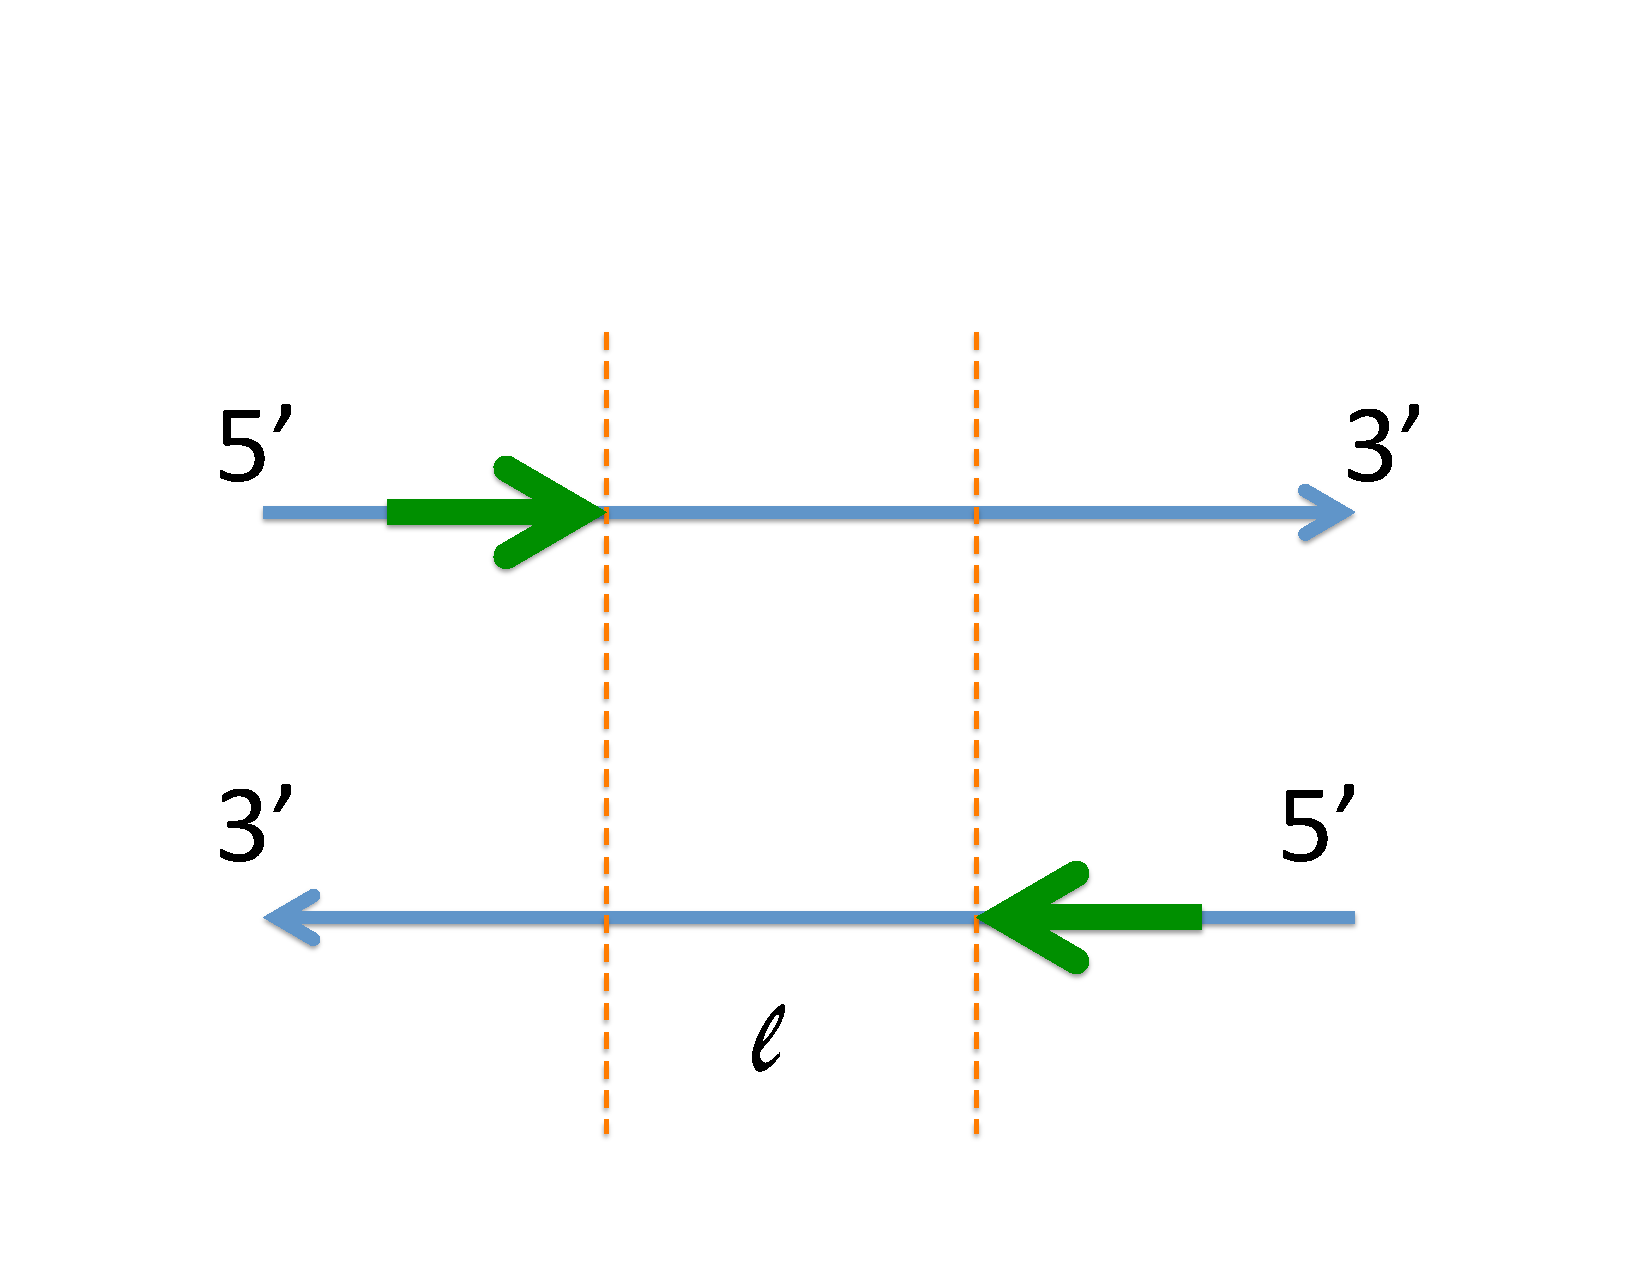
\includegraphics[width=6in]{./bioinformatics/pics/bowtie_example}
\caption{An example of Bowtie, as it tries to align a subsequence in a DNA sequence with another subsequence in another DNA sequence.}
\label{fig:BowtieExample}
\end{figure}

An example of DNA sequences being read by {\tt Bowtie} is shown in Figure \ref{fig:BowtieExample}. \\


Separate the reads into different classes, especially for genomes with lots of single nucleotide polymorphism (SNPS) $\rightarrow$ lots of inversion that need to be sorted.













%%%%%%%%%%%%%%%%%%%%%%%%%%%%%%%%%%%%%%%%%%%%%%
\section{SAM File Format}
\label{sec:SAMFileFormat}

The second field of the {\tt SAM} file format indicates various information about the alignment and pairing. It indicates the call of a proper read, or align read. The majority of the reads don't map well because we are mapping only to the smallest chromosome of the species. The {\it Neurospora crassa} species has 7 chromosomes\dots\ Without paired reads, the numbers are different. \\

Some calculations to determine such information is demonstrated as follows: \vspace{-0.3cm}
\begin{enumerate} \itemsep -4pt
\item 77 = 64 + 8 + 4 + 1
\item 141 = 128 + 8 + 4 + 1
\item 163 = 128 + 32 + 2 + 1. Properly aligned.
\item 83 = 64 + 16 + 2 + 1
\item 99 = 64 + 32 + 2+ 1
\end{enumerate}

Convert {\tt SAM} files to {\tt BAM} files, which are faster to read. {\tt SAM} files are written according to when they (i.e., the subsequences) are found/read; that is, they are written as the subsequences are found. On the other hand, the {\tt BAM} files can be sorted according to their coordinates of the beginning (and, hence, the end) of the subsequences; {\it verify this!!!}. These {\tt BAM} files are sorted from left to right. For control



















%%%%%%%%%%%%%%%%%%%%%%%%%%%%%%%%%%%%%%%%%
%	Questions
%%%%%%%%%%%%%%%%%%%%%%%%%%%%%%%%%%%%%%%%%%%%%%
\chapter{Questions}
\label{chp:Questions}



Questions: \vspace{-0.3cm}
\begin{enumerate} \itemsep -4pt
\item Are sequences in the NCBI database either DNA or transcript sequences?
\item 
\item 
\item 
\item 
\item 
\item 
\item 
\item 
\item 
\item 
\item 
\item 
\item 
\item 
\end{enumerate}





















%%%%%%%%%%%%%%%%%%%%%%%%%%%%%%%%%%%%%%%%%%%%%
%%%%%%%%%%%%%%%%%%%%%%%%%%%%%%%%%%%%%%%%%%%%%
%
%	End of document
%
%	Inserting references
%
%%%%%%%%%%%%%%%%%%%%%%%%%%%%%%%%%%%%%%%%%%%%%
%%%%%%%%%%%%%%%%%%%%%%%%%%%%%%%%%%%%%%%%%%%%%
%	Beginning of BACK MATTER: bibliography, indexes and colophon
%\backmatter
\appendix

{\linespread{1}
\bibliographystyle{plain}
%\bibliography{./references/references}
\bibliography{/data/research/antipastobibtex/references}
\addcontentsline{toc}{chapter}{Bibliography}
}
\end{document}
